\documentclass[tikz,border=5pt]{standalone}
\usepackage{tikz}
\usetikzlibrary{positioning,fit,backgrounds,calc,shapes.geometric}
\usepackage{graphicx}
\usepackage{xcolor}

\definecolor{gitopsblue}{RGB}{51,108,229}
\definecolor{manualgray}{RGB}{102,102,102}
\definecolor{driftred}{RGB}{229,115,115}
\definecolor{okgreen}{RGB}{76,175,80}
\definecolor{metricyellow}{RGB}{251,192,45}

\begin{document}
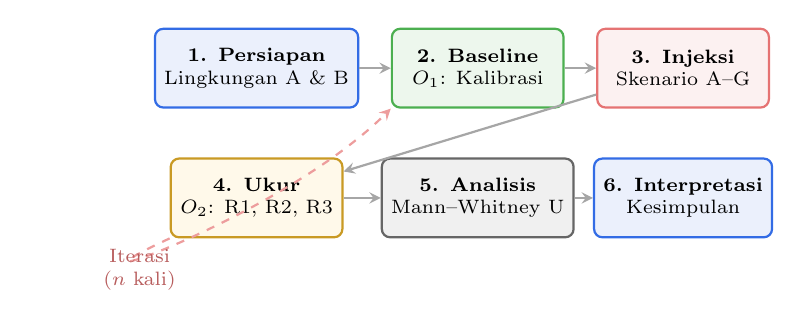
\begin{tikzpicture}[
    node distance=0.48cm and 0.42cm,
    box/.style={rectangle, rounded corners=3pt, draw=gray!60, fill=white,
                minimum width=2.18cm, minimum height=1.0cm, align=center,
                line width=0.8pt, font=\scriptsize},
    arrow/.style={->, >=stealth, line width=0.8pt, draw=gray!70},
    looparrow/.style={->, >=stealth, line width=0.8pt, draw=driftred!70, dashed}
]

\node[box, draw=gitopsblue, fill=gitopsblue!10] (s1) {
    \textbf{1. Persiapan}\\
    Lingkungan A \& B
};
\node[box, draw=okgreen, fill=okgreen!10, right=0.4cm of s1] (s2) {
    \textbf{2. Baseline}\\
    $O_1$: Kalibrasi
};
\node[box, draw=driftred, fill=driftred!10, right=0.4cm of s2] (s3) {
    \textbf{3. Injeksi}\\
    Skenario A--G
};

\node[box, draw=metricyellow!80!black, fill=metricyellow!10, below=0.62cm of s1] (s4) {
    \textbf{4. Ukur}\\
    $O_2$: R1, R2, R3
};
\node[box, draw=manualgray, fill=manualgray!10, below=0.62cm of s2] (s5) {
    \textbf{5. Analisis}\\
    Mann--Whitney U
};
\node[box, draw=gitopsblue, fill=gitopsblue!10, below=0.62cm of s3] (s6) {
    \textbf{6. Interpretasi}\\
    Kesimpulan
};

\draw[arrow] (s1) -- (s2);
\draw[arrow] (s2) -- (s3);
\draw[arrow] (s3) -- (s4);
\draw[arrow] (s4) -- (s5);
\draw[arrow] (s5) -- (s6);

\draw[looparrow] (s4.south west) to[out=205, in=225, looseness=1.55]
    node[below left, font=\scriptsize, text=driftred!80!black, align=center] {Iterasi\\($n$ kali)} (s2.south west);

\end{tikzpicture}
\end{document}
